\section{Auswertung}
\label{sec:Auswertung}
%Tabelle der gemessenen Temperaturen 
\begin{table}
	\centering
	\sisetup{table-format=2.3}
	\begin{tabular}{S[table-format=1.2] S[table-format=1.3] S[table-format=1.3] }
	\toprule
	\multicolumn{1}{c}{Zeit} & {Temperaturen} \\
	{$t/\:\si{\min}$} & {$T_1/\:\si{\kelvin}$} & {${T_2}/\:\si{\kelvin}$} \\
	\midrule

 0 & 294.45 & 294.45 \\
 1 & 295.35 & 294.45 \\
 2 & 296.15 & 294.35 \\
 3 & 297.45 & 293.45 \\
 4 & 299.05 & 292.05 \\
 5 & 300.85 & 290.25 \\
 6 & 302.95 & 288.25 \\
 7 & 304.85 & 286.45 \\
 8 & 306.85 & 284.65 \\
 9 & 308.65 & 282.85 \\
10 & 310.55 & 281.15 \\
11 & 312.25 & 279.45 \\
12 & 314.05 & 277.75 \\
13 & 315.65 & 276.35 \\
14 & 317.35 & 274.95 \\
15 & 318.85 & 273.95 \\
16 & 320.35 & 273.35 \\
17 & 321.75 & 272.85 \\
18 & 322.95 & 272.45 \\
19 & 324.15 & 272.05 \\
	\bottomrule
	\end{tabular}
	\caption{Zeitabhängige Messung der Temperaturen $T_1$ und $T_2$.}
	\label{tab:Temperaturverlauf}
\end{table}

Die gemessenen Temperaturen $T_1$ (rot) und $T_2$ (blau) der Reservoire werden gegen die Zeit $t$ aufgetragen, um einen ersten Eindruck des Temperaturverlaufes innerhalb der Reservoire zu gewinnen. Dabei ist Reservoir $R_1$ das Behältnis, welches die Wärmemenge $\mathup{d}Q_1$ aufnimmt und sich dabei erhitzt; $R_2$ (blau) bezeichnet das kälter werdende Reservoir.  Werden die Verläufe in einem gemeinsamen Diagramm dargestellt, so lassen sich diese untereinander vergleichen. 
\newpage
\begin{figure}
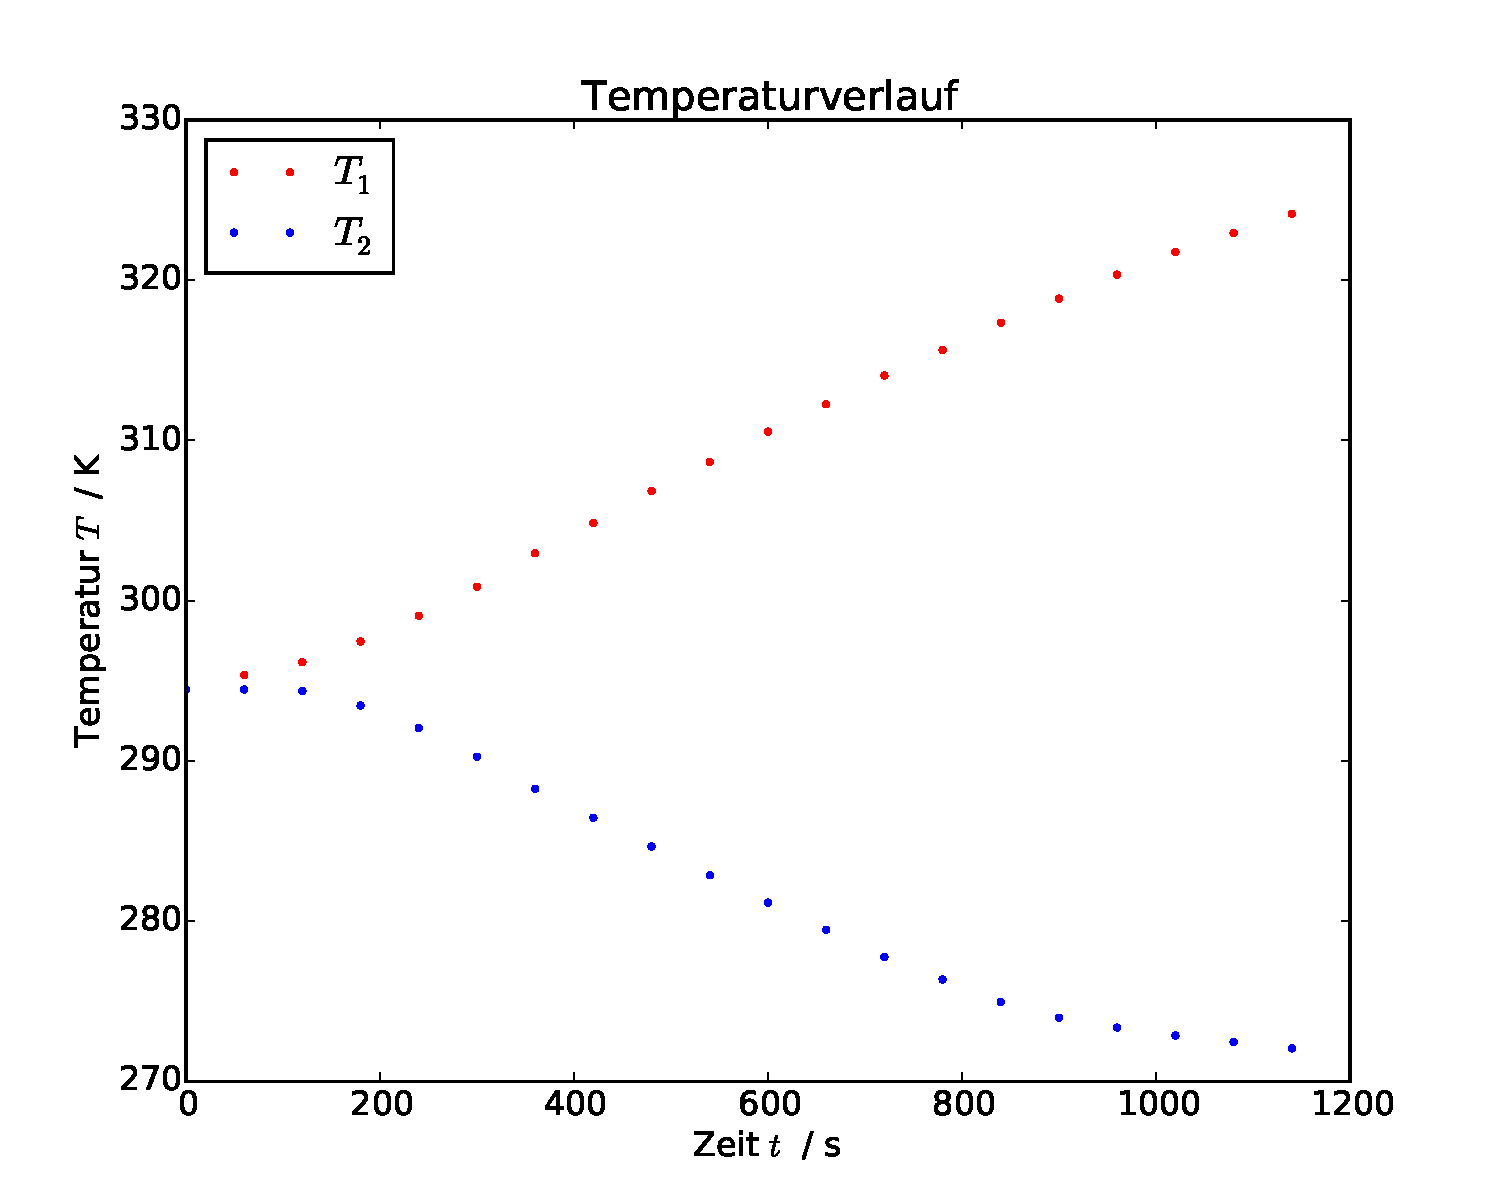
\includegraphics[width=\textwidth]{Bilder/Temperaturverlauf.pdf}
	\caption{Entwicklung der Wassertemperatur in den Reservoiren $\mathup{R_1}$ und $\mathup{R_2}$.}
	\label{fig:temperaturverlauf}
\end{figure}


Entgegen der Anweisung der Anleitung werden die Verläufe nicht durch eine nicht - lineare Ausgleichsrechnung mit
\begin{equation}
	T_i(t)=A_i t² + B_i t + C_i , i=1,2
	\label{eq:t-verlauf_Grad2}
\end{equation}
 -- einem Polynom zweiten Grades mit den Konstanten $A$, $B$ und $C$ -- genähert. Trotz zweiter Ordnung erscheint der Fit annähernd linear. Da schon anhand der Messwerte zu erkennen ist, dass diese einen Wendepunkt aufweisen wird ein Polynom dritten Grades benutzt; die Messwerte liegen deutlich weniger von der Näherung entfernt ( vgl. Abbildung 2, 3).

\begin{equation}
	T_i(t)=A_i t³ + B_i t² + C_i t + D_i , i=1,2
	\label{eq:t-verlauf_Grad3}
\end{equation}
\newpage
\begin{figure}
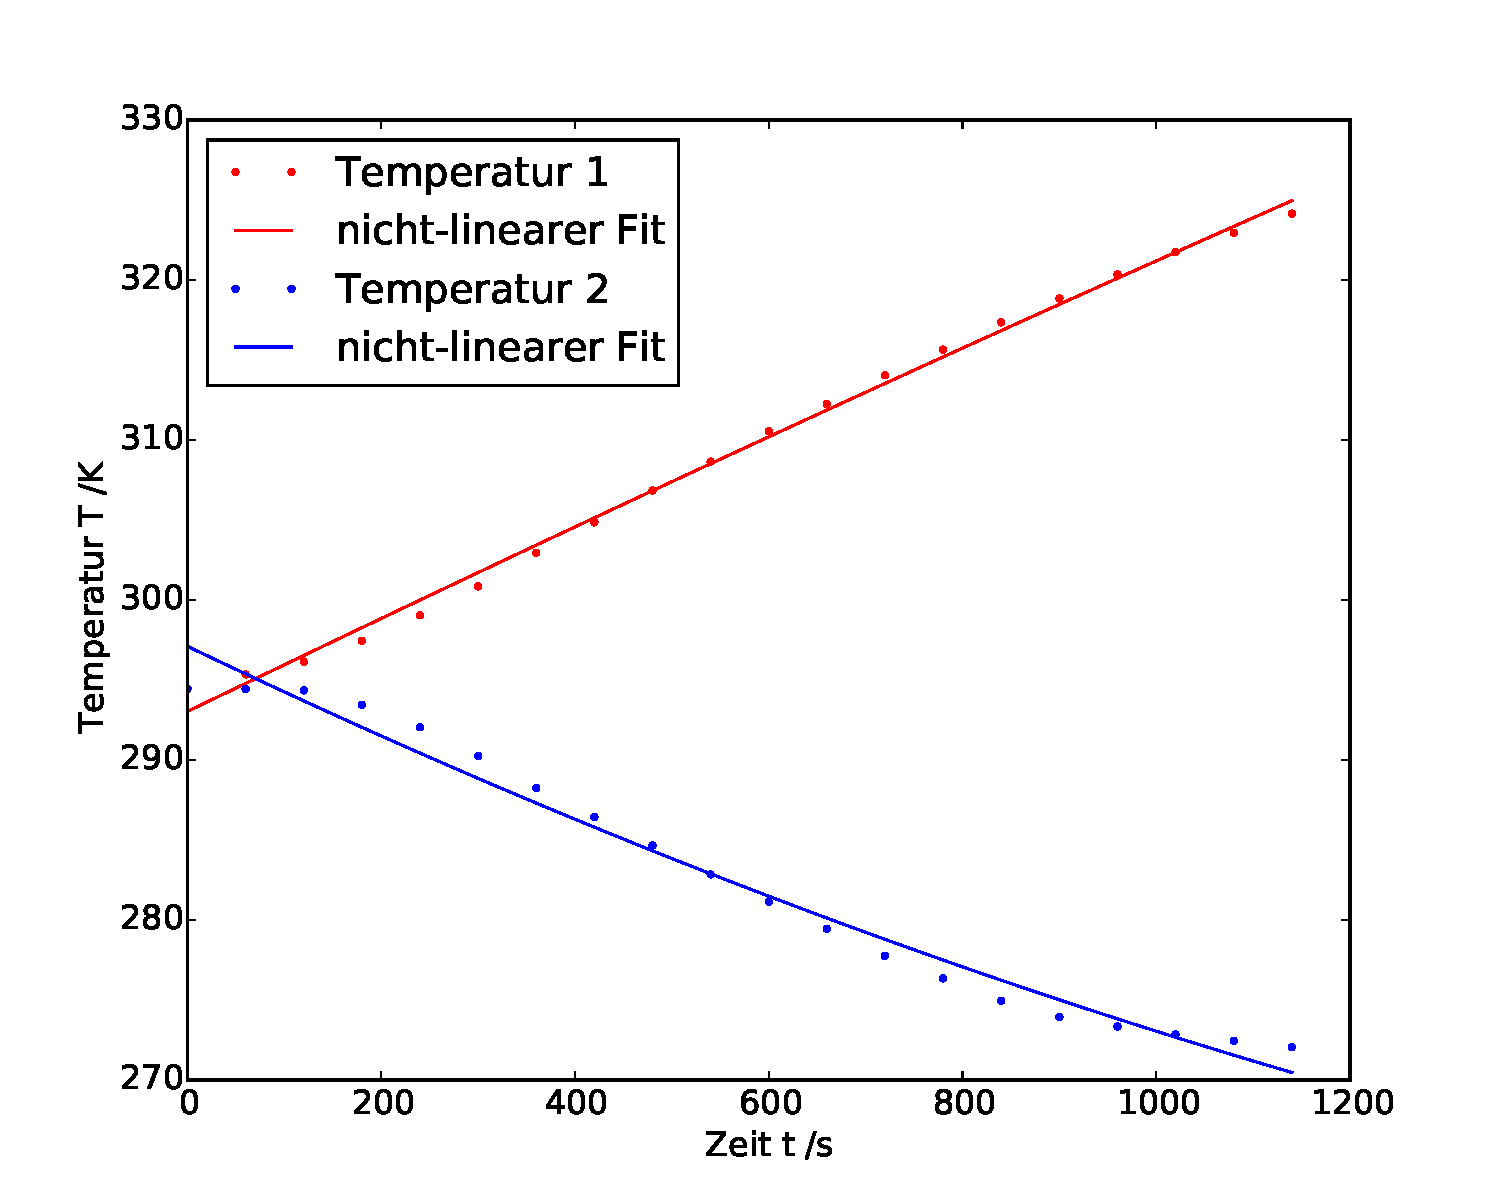
\includegraphics[width=\textwidth]{Bilder/Temperaturfit_Grad2.pdf}
	\caption{Annäherung der Kurven durch ein Polynom zweiter Ordnung.}
\end{figure}

\begin{figure}
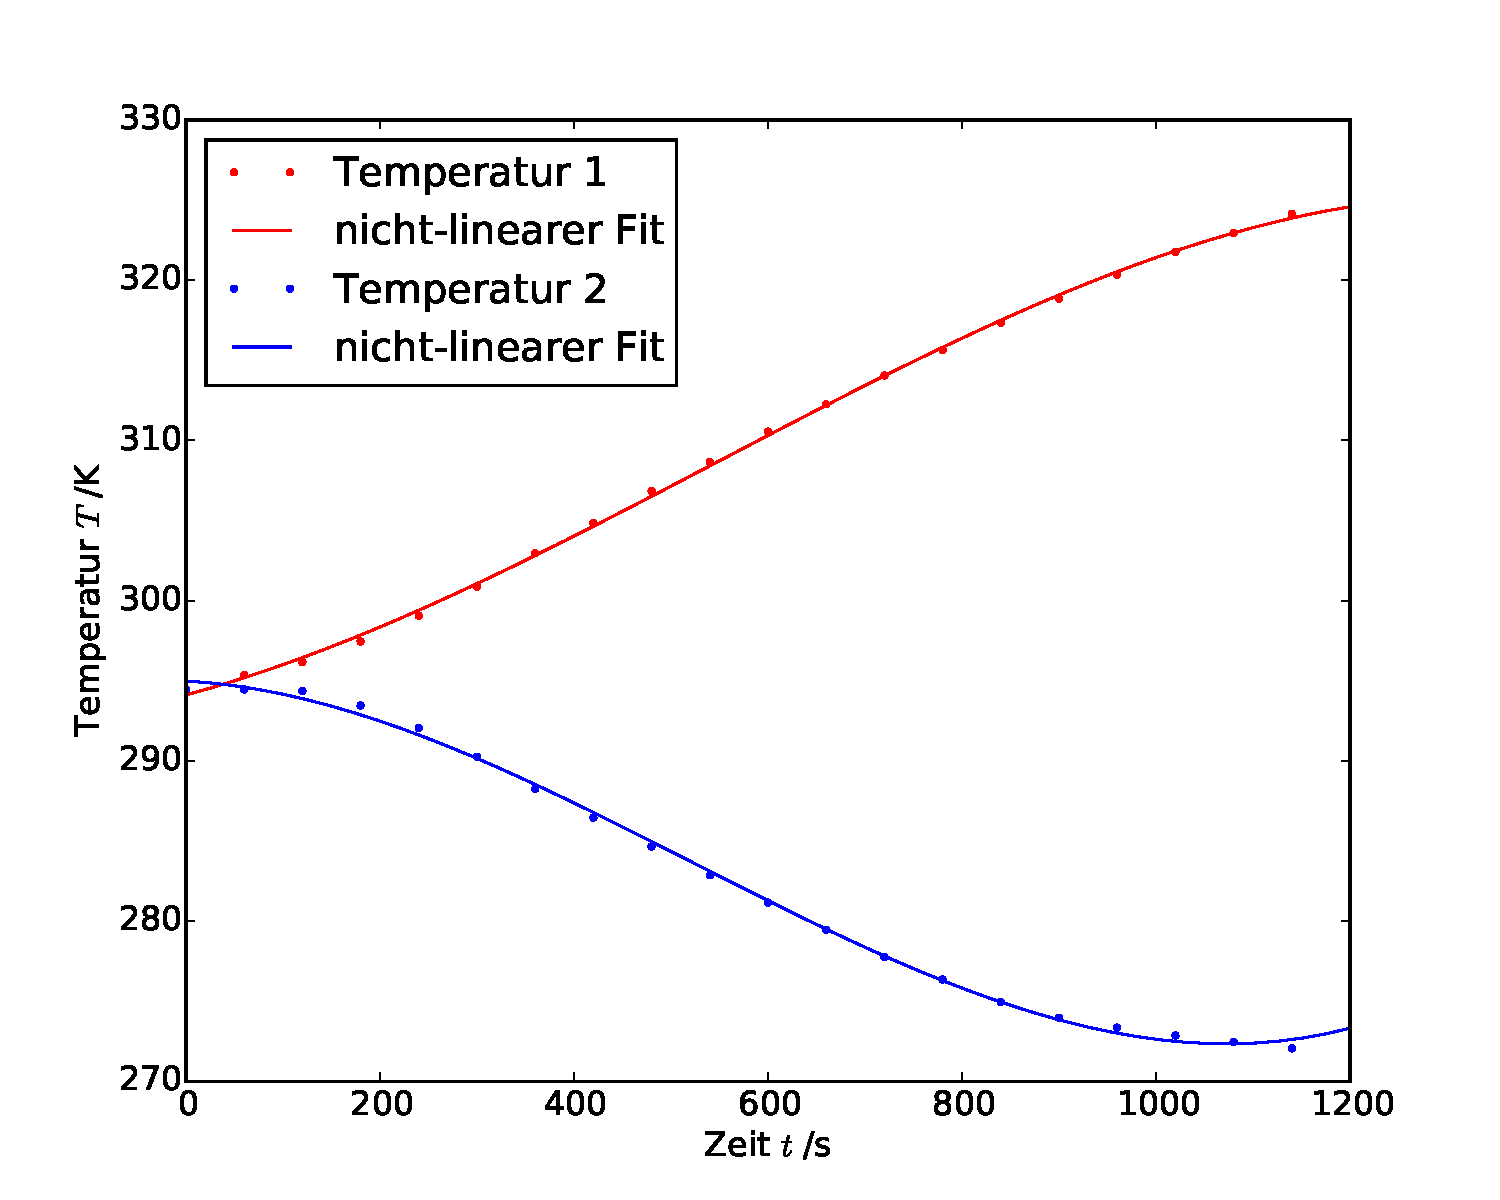
\includegraphics[width=\textwidth]{Bilder/Temperaturfit.pdf}
	\caption{Annäherung der Kurven durch ein Polynom dritter Ordnung.}
\end{figure}
\newpage
Es ergeben sich für $T_1(t)$ und $T_2(t)$ die Koeffizienten 
\begin{equation}
\begin{split}
A_1&=(-17.1705895195\pm1.7899858311)10⁻⁹\si{\kelvin\per{\second}³}\\
B_1&=(28.2367366738\pm3.10787542417)10⁻⁶\si{\kelvin\per{\second}²}\\
C_1&=(0.0162347592968\pm0.00150160292315)\si{\kelvin\per{\second}}\\
D_1&=(294.111603517\pm0.19259208147)\si{\kelvin}
\end{split}
\end{equation}
und
\begin{equation}
\begin{split}
A_2&=(33.855559517\pm2.46581851787)10⁻⁹\si{\kelvin\per{\second}³}\\
B_2&=(-52.9611716421\pm4.28129424103)10⁻⁶\si{\kelvin\per{\second}²}\\
C_2&=(-0.00325557626607\pm0.00206855306032)\si{\kelvin\per{\second}}\\
D_2&=(294.977609839\pm0.265307963098)\si{\kelvin}.
\end{split}
\end{equation}

Um den Differentialqutionenten $\frac{\mathup{d}T_i}{\mathup{d}t}$ mit $i=1,2$ für verschiedene Zeiten $t_k$ mit $k=1,...,4$ bestimmen zu können, wird die Funktion $T_i(t)$ nach der Zeit $t$ abgeleitet:

\begin{equation}
\frac{\mathup{d}T_i}{\mathup{d}t}= 3A_it²+2B_it+C_i.
\label{ableitung}
\end{equation}

\begin{table}
	\centering
	
	\begin{tabular}{S S S}
	\toprule
	\multicolumn{1}{c}{Zeit} & \multicolumn{2}{c}{Differentialquotienten} \\
	{$t/\:\si{\second}$} & {$\frac{\mathup{d}T_1}{\mathup{d}t}/\:\si{\kelvin{\per\second}}$} & {$\frac{\mathup{d}T_2}{\mathup{d}t}/\:\si{\kelvin{\per\second}}$}\\
	\midrule
 120 & 0.022 $\pm$\:\:46.222   & 0.022 $\pm$\:\:63.674  \\
 480 & 0.032 $\pm$ 184.888   & 0.032 $\pm$ 254.696  \\
 840 & 0.027 $\pm$ 323.555   & 0.027 $\pm$ 445.717  \\
1080 & 0.017 $\pm$ 415.999   & 0.017 $\pm$ 573.065  \\
	\bottomrule
	\end{tabular}
	\caption{Die Differentialqutienten von $T_1$ und $T_2$ zu vier verschiedenen Zeiten $t_k$, berechnet nach Gleichung \eqref{ableitung}.}
	\label{tab:differentialquotienten}
\end{table}

%erst gegen Ende.
Vor Beginn der Messung zur Zeit $t=0$ haben wie in Kapitel \ref{sec:Durchfuehrung} beschrieben beide Behälter dieselbe Temperatur: $T_1(0)=T_2(0)=21.3\si{\celsius}=294.45\si{\kelvin}$.


